\documentclass{ximera}

%\usepackage{todonotes}

\newcommand{\todo}{}

\usepackage{esint} % for \oiint
\graphicspath{
  {./}
  {ximeraTutorial/}
}

\newcommand{\mooculus}{\textsf{\textbf{MOOC}\textnormal{\textsf{ULUS}}}}

\usepackage{tkz-euclide}
\tikzset{>=stealth} %% cool arrow head
\tikzset{shorten <>/.style={ shorten >=#1, shorten <=#1 } } %% allows shorter vectors

\usetikzlibrary{backgrounds} %% for boxes around graphs
\usetikzlibrary{shapes,positioning}  %% Clouds and stars
\usetikzlibrary{matrix} %% for matrix
\usepgfplotslibrary{polar} %% for polar plots
\usetkzobj{all}
\usepackage[makeroom]{cancel} %% for strike outs
%\usepackage{mathtools} %% for pretty underbrace % Breaks Ximera
\usepackage{multicol}
\usepackage{pgffor} %% required for integral for loops


%% http://tex.stackexchange.com/questions/66490/drawing-a-tikz-arc-specifying-the-center
%% Draws beach ball 
\tikzset{pics/carc/.style args={#1:#2:#3}{code={\draw[pic actions] (#1:#3) arc(#1:#2:#3);}}}



\usepackage{array}
\setlength{\extrarowheight}{+.1cm}   
\newdimen\digitwidth
\settowidth\digitwidth{9}
\def\divrule#1#2{
\noalign{\moveright#1\digitwidth
\vbox{\hrule width#2\digitwidth}}}





\newcommand{\RR}{\mathbb R}
\newcommand{\R}{\mathbb R}
\newcommand{\N}{\mathbb N}
\newcommand{\Z}{\mathbb Z}

\newcommand{\sagemath}{\textsf{SageMath}}


%\renewcommand{\d}{\,d\!}
\renewcommand{\d}{\mathop{}\!d}
\newcommand{\dd}[2][]{\frac{\d #1}{\d #2}}
\newcommand{\pp}[2][]{\frac{\partial #1}{\partial #2}}
\renewcommand{\l}{\ell}
\newcommand{\ddx}{\frac{d}{\d x}}

\newcommand{\zeroOverZero}{\ensuremath{\boldsymbol{\tfrac{0}{0}}}}
\newcommand{\inftyOverInfty}{\ensuremath{\boldsymbol{\tfrac{\infty}{\infty}}}}
\newcommand{\zeroOverInfty}{\ensuremath{\boldsymbol{\tfrac{0}{\infty}}}}
\newcommand{\zeroTimesInfty}{\ensuremath{\small\boldsymbol{0\cdot \infty}}}
\newcommand{\inftyMinusInfty}{\ensuremath{\small\boldsymbol{\infty - \infty}}}
\newcommand{\oneToInfty}{\ensuremath{\boldsymbol{1^\infty}}}
\newcommand{\zeroToZero}{\ensuremath{\boldsymbol{0^0}}}
\newcommand{\inftyToZero}{\ensuremath{\boldsymbol{\infty^0}}}



\newcommand{\numOverZero}{\ensuremath{\boldsymbol{\tfrac{\#}{0}}}}
\newcommand{\dfn}{\textbf}
%\newcommand{\unit}{\,\mathrm}
\newcommand{\unit}{\mathop{}\!\mathrm}
\newcommand{\eval}[1]{\bigg[ #1 \bigg]}
\newcommand{\seq}[1]{\left( #1 \right)}
\renewcommand{\epsilon}{\varepsilon}
\renewcommand{\phi}{\varphi}


\renewcommand{\iff}{\Leftrightarrow}

\DeclareMathOperator{\arccot}{arccot}
\DeclareMathOperator{\arcsec}{arcsec}
\DeclareMathOperator{\arccsc}{arccsc}
\DeclareMathOperator{\si}{Si}
\DeclareMathOperator{\proj}{\vec{proj}}
\DeclareMathOperator{\scal}{scal}
\DeclareMathOperator{\sign}{sign}


%% \newcommand{\tightoverset}[2]{% for arrow vec
%%   \mathop{#2}\limits^{\vbox to -.5ex{\kern-0.75ex\hbox{$#1$}\vss}}}
\newcommand{\arrowvec}{\overrightarrow}
%\renewcommand{\vec}[1]{\arrowvec{\mathbf{#1}}}
\renewcommand{\vec}{\mathbf}
\newcommand{\veci}{{\boldsymbol{\hat{\imath}}}}
\newcommand{\vecj}{{\boldsymbol{\hat{\jmath}}}}
\newcommand{\veck}{{\boldsymbol{\hat{k}}}}
\newcommand{\vecl}{\boldsymbol{\l}}
\newcommand{\uvec}[1]{\mathbf{\hat{#1}}}
\newcommand{\utan}{\mathbf{\hat{t}}}
\newcommand{\unormal}{\mathbf{\hat{n}}}
\newcommand{\ubinormal}{\mathbf{\hat{b}}}

\newcommand{\dotp}{\bullet}
\newcommand{\cross}{\boldsymbol\times}
\newcommand{\grad}{\boldsymbol\nabla}
\newcommand{\divergence}{\grad\dotp}
\newcommand{\curl}{\grad\cross}
%\DeclareMathOperator{\divergence}{divergence}
%\DeclareMathOperator{\curl}[1]{\grad\cross #1}
\newcommand{\lto}{\mathop{\longrightarrow\,}\limits}

\renewcommand{\bar}{\overline}

\colorlet{textColor}{black} 
\colorlet{background}{white}
\colorlet{penColor}{blue!50!black} % Color of a curve in a plot
\colorlet{penColor2}{red!50!black}% Color of a curve in a plot
\colorlet{penColor3}{red!50!blue} % Color of a curve in a plot
\colorlet{penColor4}{green!50!black} % Color of a curve in a plot
\colorlet{penColor5}{orange!80!black} % Color of a curve in a plot
\colorlet{penColor6}{yellow!70!black} % Color of a curve in a plot
\colorlet{fill1}{penColor!20} % Color of fill in a plot
\colorlet{fill2}{penColor2!20} % Color of fill in a plot
\colorlet{fillp}{fill1} % Color of positive area
\colorlet{filln}{penColor2!20} % Color of negative area
\colorlet{fill3}{penColor3!20} % Fill
\colorlet{fill4}{penColor4!20} % Fill
\colorlet{fill5}{penColor5!20} % Fill
\colorlet{gridColor}{gray!50} % Color of grid in a plot

\newcommand{\surfaceColor}{violet}
\newcommand{\surfaceColorTwo}{redyellow}
\newcommand{\sliceColor}{greenyellow}




\pgfmathdeclarefunction{gauss}{2}{% gives gaussian
  \pgfmathparse{1/(#2*sqrt(2*pi))*exp(-((x-#1)^2)/(2*#2^2))}%
}


%%%%%%%%%%%%%
%% Vectors
%%%%%%%%%%%%%

%% Simple horiz vectors
\renewcommand{\vector}[1]{\left\langle #1\right\rangle}


%% %% Complex Horiz Vectors with angle brackets
%% \makeatletter
%% \renewcommand{\vector}[2][ , ]{\left\langle%
%%   \def\nextitem{\def\nextitem{#1}}%
%%   \@for \el:=#2\do{\nextitem\el}\right\rangle%
%% }
%% \makeatother

%% %% Vertical Vectors
%% \def\vector#1{\begin{bmatrix}\vecListA#1,,\end{bmatrix}}
%% \def\vecListA#1,{\if,#1,\else #1\cr \expandafter \vecListA \fi}

%%%%%%%%%%%%%
%% End of vectors
%%%%%%%%%%%%%

%\newcommand{\fullwidth}{}
%\newcommand{\normalwidth}{}



%% makes a snazzy t-chart for evaluating functions
%\newenvironment{tchart}{\rowcolors{2}{}{background!90!textColor}\array}{\endarray}

%%This is to help with formatting on future title pages.
\newenvironment{sectionOutcomes}{}{} 



%% Flowchart stuff
%\tikzstyle{startstop} = [rectangle, rounded corners, minimum width=3cm, minimum height=1cm,text centered, draw=black]
%\tikzstyle{question} = [rectangle, minimum width=3cm, minimum height=1cm, text centered, draw=black]
%\tikzstyle{decision} = [trapezium, trapezium left angle=70, trapezium right angle=110, minimum width=3cm, minimum height=1cm, text centered, draw=black]
%\tikzstyle{question} = [rectangle, rounded corners, minimum width=3cm, minimum height=1cm,text centered, draw=black]
%\tikzstyle{process} = [rectangle, minimum width=3cm, minimum height=1cm, text centered, draw=black]
%\tikzstyle{decision} = [trapezium, trapezium left angle=70, trapezium right angle=110, minimum width=3cm, minimum height=1cm, text centered, draw=black]


\title{Function Questions}

\begin{document}

\begin{abstract}
%Stuff can go here later if we want!
\end{abstract}

\maketitle





\textbf{Pairs in a Function} \\


\begin{center}
\textbf{$(domainItem, functionName(domainItem))$}
\end{center}

The left coordinate is a domain item and the right coordinate is THE codomain partner, or THE value of the function at this domain item.
\quad \\

\begin{example}
\quad \\
$(Amy Ward, MartinIceCream(Amy Ward))$ is a pair in the MartinIceCream function. Amy Ward is certainly paired with $MartinIceCream(Amy Ward)$, because $MartinIceCream(Amy Ward)$ represents the codomain item paired with Amy Ward.

If we take the time to sift through the MartinIceCream table, then we might discover that Amy Ward is paired with Cookie Dough.  $(Amy Ward, Cookie Dough)$ is a pair in the MartinIceCream function. 

In fact, $(Amy Ward, MartinIceCream(Amy Ward))$ and $(Amy Ward, Cookie Dough)$ are the same pair (just written in two different ways), because $MartinIceCream(Amy Ward) = Cookie Dough$.

The equation is just our way of saying that the two expressions represent the same value.        

\end{example}


\quad \\



\textbf{Questions} \\
\quad \\

Superficially, a function is a package of pairs, which gives us just two types of questions to ask about functions.
\quad \\

\underline{TYPE I} \\
You might know the domain item and ask about its codomain partner. 

\begin{center}
(Sila Vane, flavor)
\end{center}


In this scenario, we usually just refer to the codomain partner via function notation. "flavor" is representing Sila Vane's codomain partner, so let's just write that:
\begin{center}
flavor = $MartinIceCream(Sila Vane)$
\end{center}

Here we know the domain item, Silas Vane, and we are representing the codomain partner, i.e. the value of MartinIceCream at Silas Vane.  

People throw around the word "evaluate" in this scenario when they might want someone to sift through the pairs and identify the exact codomain value for $MartinIceCream(Sila Vane)$.

\quad \\
\underline{TYPE II} \\
\quad \\

On the other hand, you might know the codomain item and ask about its domain partner.
\begin{center}
(name, Strawberry)
\end{center}

In this scenario we know the value of the function, which means we can use an equation to describe the value of the function.
\begin{center}
$MartinIceCream(name)$ = Strawberry 
\end{center}


This is an equation.  It has a variable, which is representing domain items. Any domain item which can replace the variable and create a true statement about the function is called a solution.  Naturally, people throw around the word "solve" in this scenario. The solutions are the domain items that complete the pairs in question.

Here the variable name could be representing Kyra Hogan, Brady Delter, or Samantha Devon.


$name \in \{ Kyra Hogan, Brady Delter, Samantha Devon \}$

This is called the solution set of the equation.


\quad \\

\begin{itemize}
\item \textit{If you know the domain item in a pair, then there can only be one range partner.  That is how a function works.}

\item \textit{If you know the range item in the pair, then there could be multiple domain partners. The special rule of functions only only talks about the domain in pairs.}
\end{itemize}


\quad \\

\textbf{More Pieces to a Function} \\

As we saw in the MartinIceCream function each domain name had to appear in an ordered pair, but not every codomain items has to appear in an ordered pair. The rule for functions only affects the domain. Some of the codomain items are in ordered pairs and some are not. We might as well give a name to the subset of codomain items that do appear in ordered pairs.

\begin{definition}
\quad \\
The subset of codomain items that actually appear in an ordered pair is called the \textbf{Range} of the function.
\end{definition}


\begin{example}
The range of the MartinIceCream function is 
\{ Chocolate, Cookie Dough, Vanilla, Strawberry, Mint Chocolate, Chocolate Chip, Peach \}.

These are the codomain items that actually appear in an ordered pair of the function.  The range of the MartinIceCream function doesn't include Toffee, Pistachio, or Butter Pecan, because they did not appear in any ordered pair.
\end{example}




\textbf{Martin Ice Cream function} \\
\begin{center}

\begin{tabular}{|l|l|l|l|}
\hline
Kindergartner & Ice Cream & Kindergartner & Ice Cream \\\hline 
Johnny Warner & Chocolate & Bridget London & Mint Chocolate \\\hline 
Sara Turns & Cookie Dough & Shawn Trails & Chocolate \\\hline 
Lisa O'Reilly & Vanilla & Quinn Wallace & Chocolate \\\hline 
Martha Reater & Vanilla & Brady Delter & Strawberry \\\hline 
Ashley Teasley & Cookie Dough & Amy Ward & Cookie Dough \\\hline 
Mark Tortan & Chocolate & Micah McCain & Vanilla \\\hline 
Silas Vane & Vanilla & Bobby Post & Chocolate Chip \\\hline 
Kyra Hogan & Strawberry & Leah Korch & Peach \\\hline 
Steven Stokes & Chocolate & Samantha Devon & Strawberry \\\hline 
Emeka Simpson & Vanilla & Charlie Allston & Chocolate \\\hline 
\end{tabular}

\end{center}

\quad \\


\begin{question}
Evaluate $MartinIceCream(Steven Stokes)$.
\begin{multipleChoice}
\choice{Vanilla}
\choice[correct]{Chocolate}
\choice{Strawberry}
\choice{Mint Chocolate}
\end{multipleChoice}
\end{question}


\begin{question}
Solve $MartinIceCream(Steven Stokes)$ = Peach.
\begin{multipleChoice}
\choice{Bridget London}
\choice{Samantha Devon}
\choice{Sarah Turns}
\choice[correct]{Leah Korch}
\end{multipleChoice}
\end{question}



\begin{question}
Which is not a solution of $MartinIceCream(name)$ = Chocolate.
\begin{multipleChoice}
\choice[correct]{Charlie Allston}
\choice{Bridget London}
\choice{Bobby Post}
\choice{Steven Stokes}
\end{multipleChoice}
\end{question}



\begin{question}
$MartinIceCream(MarkTortan) = MartinIceCream(Johnny Warner)$
\begin{multipleChoice}
\choice[correct]{True}
\choice{False}
\end{multipleChoice}
\end{question}




\begin{question}
The equation $MartinIceCream(name)$ = Strawberry describes which set?
\begin{multipleChoice}
\choice{\{ Kyra Hogan, Brady Delter \}}
\choice{\{ Kyra Hogan \}}
\choice[correct]{\{ Kyra Hogan, Brady Delter, Samantha Devon \}}
\choice{not enough information}
\end{multipleChoice}
\end{question}


\quad \\

A function is a package. It contains a set called the domain, a set called the codomain, and a set or pairs gluing together the domain and codomain. The only rule is that every domain item appears in exactly one pair. Not every codomain item has to appear in a pair.  The collection of codomain items that do appear in the pairs is called the range.  The range is a subset of the codomain. 
The pairs are the most important part of a function. We have many ways of communicating these pairs. One method is simply to list them as ordered pairs with parentheses and a comma.  The ordering means that we write the domain item on the left followed by the range partner. 

\quad \\

\textbf{Other Representations} \\
So far, we are representing the function pairs via a table or by writing ordered pairings with parentheses and a comma.  This will seamlessly transfer to graphs of functions when we study them.  But, another representation is called a \textbf{map}.  A map is a drawing.  The domain is drawn showing its members. The codomain is drawn showing its members. Arrows represent the pairs.  An arrow is drawn from a domain item to its codomain (or range) partner.

\quad \\


\begin{example}
Here is a map of the function $Cone$.

\begin{image}
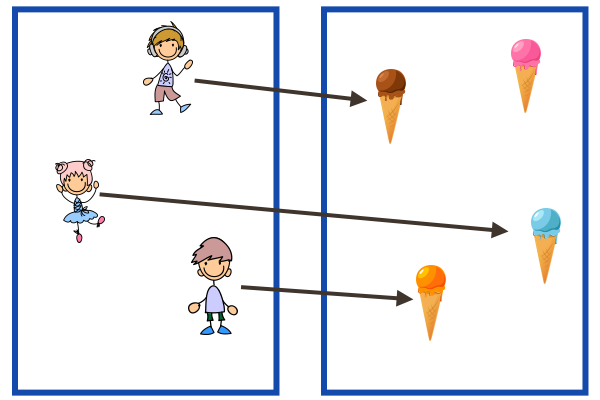
\includegraphics{pics/f_20.png}
\end{image}

\end{example}



\end{document}
